% !TeX program = xelatex
\documentclass[a4paper,10pt]{article}

% ============================================================================
% កញ្ចប់បណ្ណាល័យ (Packages) – តាមលំនាំ NGS Preah Krasang (ls_plan.tex)
% បរិបទ៖ គ្មានស្លាយ LCD និងគ្មានម៉ាស៊ីនគិតលេខ — ប្រើសន្លឹកកិច្ចការសិស្ស (ស-ខ្មៅ) និងក្ដារខៀនជាគោល
% ============================================================================
\usepackage[a4paper, left=0.95cm, right=0.95cm, top=0.85cm, bottom=0.92cm, footskip=0.52cm]{geometry}
\usepackage{amsmath}
\usepackage{unicode-math}
\usepackage{fontspec}
\usepackage{array, longtable, multirow, colortbl}
\usepackage[table]{xcolor}
\usepackage{enumitem}
\usepackage{pifont}
\usepackage{fancyhdr}
\usepackage{tikz}
\usetikzlibrary{calc, arrows.meta, angles, quotes, decorations.markings, decorations.pathreplacing, patterns, babel}

\makeatletter
\let\@expl@@@mark@update@singlecol@structures@@\relax
\makeatother

\providecommand{\NGSFindFonts}{%
  \IfFileExists{C:/Windows/Fonts/cambria.ttc}{%
    \def\NGSSysPath{C:/Windows/Fonts/}%
    \def\NGSUserPath{C:/Users/KIT/AppData/Local/Microsoft/Windows/Fonts/}%
  }{%
    \IfFileExists{./fonts/KhmerOSsiemreap.ttf}{\def\NGSSysPath{./fonts/}\def\NGSUserPath{./fonts/}}{%
    \IfFileExists{../fonts/KhmerOSsiemreap.ttf}{\def\NGSSysPath{../fonts/}\def\NGSUserPath{../fonts/}}{%
    \IfFileExists{../../fonts/KhmerOSsiemreap.ttf}{\def\NGSSysPath{../../fonts/}\def\NGSUserPath{../../fonts/}}{%
    \IfFileExists{../../../fonts/KhmerOSsiemreap.ttf}{\def\NGSSysPath{../../../fonts/}\def\NGSUserPath{../../../fonts/}}{%
    \IfFileExists{../../../../fonts/KhmerOSsiemreap.ttf}{\def\NGSSysPath{../../../../fonts/}\def\NGSUserPath{../../../../fonts/}}{%
    \IfFileExists{../../../../../fonts/KhmerOSsiemreap.ttf}{\def\NGSSysPath{../../../../../fonts/}\def\NGSUserPath{../../../../../fonts/}}{%
    \IfFileExists{../../../../../../fonts/KhmerOSsiemreap.ttf}{\def\NGSSysPath{../../../../../../fonts/}\def\NGSUserPath{../../../../../../fonts/}}{%
      \def\NGSSysPath{../../../../../../../fonts/}\def\NGSUserPath{../../../../../../../fonts/}%
    }}}}}}}%
  }%
}
\NGSFindFonts

\setmathfont[Path={\NGSSysPath}, FontIndex=1, Scale=1.02]{cambria.ttc}
\defaultfontfeatures{Ligatures=TeX}

\setmainfont[
  Path={\NGSUserPath}, Extension=.ttf, Script=Khmer,
  BoldFont={KhmerOSsiemreap}, BoldFeatures={FakeBold=1.8},
  ItalicFont={KhmerOSsiemreap}, ItalicFeatures={FakeSlant=0.25},
  BoldItalicFont={KhmerOSsiemreap}, BoldItalicFeatures={FakeBold=1.8, FakeSlant=0.25}
]{KhmerOSsiemreap}

\newfontfamily\muol[Path={\NGSUserPath}, Extension=.ttf, Script=Khmer]{KhmerOSmuollight}
\newfontfamily\TimesEn[Path={\NGSSysPath}, Extension=.ttf, Scale=1.00, BoldFont={timesbd}, ItalicFont={timesi}, BoldItalicFont={timesbi}]{times}
\newfontfamily\NagaBold[Path={\NGSUserPath}, Extension=.ttf]{AKbalthom Naga Bold}
\newfontfamily\CalibriFont[Path={\NGSSysPath}, Extension=.ttf]{calibri}
\newfontfamily\Tacteing[Path={\NGSUserPath}]{TACTENG.TTF}
\newfontfamily\CourierBullet[Path={\NGSSysPath}, Extension=.ttf]{cour}
\newcommand{\wcirc}{{\CourierBullet\fontsize{9.5pt}{11pt}\selectfont o}}

\XeTeXlinebreaklocale "km"
\XeTeXlinebreakskip = 0pt plus 1pt minus 0.1pt

\definecolor{stepgray}{HTML}{D9D9D9}
\definecolor{headgray}{HTML}{F2F2F2}
\definecolor{boxgray}{HTML}{D9D9D9}
\definecolor{darkred}{HTML}{C00000}
\definecolor{red5e}{HTML}{FF0000}

\pagestyle{fancy}
\fancyhf{}
\renewcommand{\headrulewidth}{0pt}
\fancyfoot[R]{\CalibriFont\fontsize{11pt}{13pt}\selectfont\thepage}

\setlength{\parindent}{0pt}
\setlength{\parskip}{0pt}
\setlength{\tabcolsep}{3.8pt}

\newcolumntype{L}[1]{>{\raggedright\arraybackslash}p{#1}}
\newcolumntype{C}[1]{>{\centering\arraybackslash}p{#1}}

\newcommand{\en}[1]{{\TimesEn #1}}
\newcommand{\enbf}[1]{{\TimesEn\textbf{#1}}}
\newcommand{\unit}[1]{\,\text{\en{#1}}}
\newcommand{\fiveE}[1]{{\NagaBold\fontsize{9.5pt}{13pt}\selectfont\textcolor{red5e}{#1}}}
\newcommand{\timenote}[1]{\textcolor{darkred}{\textit{#1}}}
\newcommand{\redsub}[1]{\textcolor{darkred}{#1}}
\newcommand{\graybox}[1]{\colorbox{boxgray}{\strut\hspace{2pt}#1\hspace{2pt}}}
\newcommand{\ditem}{\tikz[baseline=-0.5ex]\fill (0,0.42ex) -- (0.42ex,0) -- (0,-0.42ex) -- (-0.42ex,0) -- cycle;\hspace{0.3em}}
\newcommand{\cnum}[1]{{\fontsize{10.5pt}{12pt}\selectfont\ding{\numexpr181+#1\relax}}\hspace{0.15em}}
\newcommand{\cfig}[1]{\par\vspace{3pt}{\centering #1\par}\vspace{3pt}}
\newcommand{\stepheader}[1]{\multicolumn{3}{|c|}{\cellcolor{stepgray}\muol #1} \\* \noalign{\hrule height 0.4pt}}
\newcommand{\khmflourish}{{\Tacteing\fontsize{36pt}{14pt}\selectfont\raisebox{-5pt}{3}}}

% ============================================================================
% ម៉ាក្រូគូសរូប TikZ ស-ខ្មៅ ១០០% សម្រាប់មេរៀន ៣.១.១ ទំហំសមាមាត្រស្រប (PROP1)
% ============================================================================

% ១. E1 Engage: រ៉ឺស័រយឺត ទល់នឹង អន្ទាក់អាយុបងប្អូន (ទំ.២៧)
\newcommand{\figEngagePROPA}{%
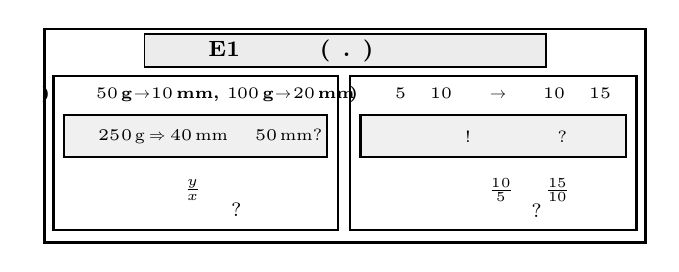
\begin{tikzpicture}[x=0.96cm, y=0.92cm, every node/.style={font=\scriptsize, text=black}]
  \draw[black, line width=0.95pt] (0,0) rectangle (7.95,2.95);
  \node[fill=gray!15, draw=black, line width=0.6pt, inner sep=2pt, font=\footnotesize\bfseries] at (3.975,2.65) {បេសកកម្ម \en{E1}៖ រ៉ឺស័រយឺត (ទំ.២៧) ទល់នឹង អន្ទាក់អាយុបងប្អូន};

  \draw[black, line width=0.8pt] (0.12,0.18) rectangle (3.88,2.30);
  \node[font=\fontsize{5.8pt}{7.6pt}\selectfont\bfseries] at (2.00,2.04) {១) រ៉ឺស័រ៖ $50\unit{g}\!\to\! 10\unit{mm}$, $100\unit{g}\!\to\! 20\unit{mm}$};
  \draw[black, line width=0.75pt, fill=gray!12] (0.26,1.18) rectangle (3.74,1.76);
  \node[font=\fontsize{5.9pt}{7.6pt}\selectfont] at (2.00,1.47) {ព្យួរ $250\unit{g} \Rightarrow 40\unit{mm}$ \;ឬ\; $50\unit{mm}$?};
  \node[align=center] at (2.00,0.62) {តើផលធៀប $\frac{y}{x}$ មានតម្លៃ\\ថេរស្មើប៉ុន្មាន?};

  \draw[black, line width=0.8pt] (4.04,0.18) rectangle (7.83,2.30);
  \node[font=\fontsize{5.8pt}{7.6pt}\selectfont\bfseries] at (5.935,2.04) {២) ប្អូន $5$ បង $10$ ឆ្នាំ $\to$ ប្អូន $10$ បង $15$ ឆ្នាំ};
  \draw[black, line width=0.75pt, fill=gray!12] (4.18,1.18) rectangle (7.69,1.76);
  \node[font=\fontsize{5.9pt}{7.6pt}\selectfont] at (5.935,1.47) {កើនទាំងពីរ! តើសមាមាត្រស្របឬទេ?};
  \node[align=center] at (5.935,0.62) {ពិនិត្យផលធៀប $\frac{10}{5}$ និង $\frac{15}{10}$\\តើស្មើគ្នាដែរឬទេ?};
\end{tikzpicture}}

% ២. E2 POE 1 & 2: តារាងរ៉ឺស័រ (ទំ.២៧) និងការប្រៀបធៀបផលធៀបថេរ
\newcommand{\figSpringPROPA}{%
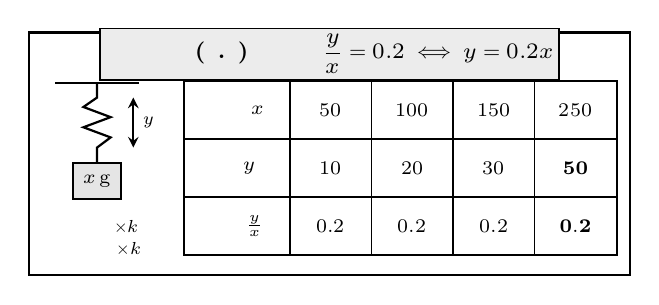
\begin{tikzpicture}[x=0.96cm, y=0.92cm, every node/.style={font=\scriptsize, text=black}]
  \draw[black, line width=0.95pt] (0,0) rectangle (7.95,3.35);
  \node[fill=gray!15, draw=black, line width=0.6pt, inner sep=2pt, font=\footnotesize\bfseries] at (3.975,3.05) {ពិសោធន៍រ៉ឺស័រ (ទំ.២៧)៖ ផលធៀបថេរ $\dfrac{y}{x} = 0.2 \iff y = 0.2x$};

  % Spring sketch on left
  \draw[black, line width=1.0pt] (0.35,2.65) -- (1.45,2.65);
  \draw[black, line width=0.8pt] (0.90,2.65) -- (0.90,2.45) -- (0.72,2.32) -- (1.08,2.18) -- (0.72,2.04) -- (1.08,1.90) -- (0.90,1.76) -- (0.90,1.55);
  \draw[black, line width=0.9pt, fill=gray!20] (0.58,1.05) rectangle (1.22,1.55);
  \node at (0.90,1.30) {$x\unit{g}$};
  \draw[<->, >=stealth, line width=0.7pt] (1.38,1.76) -- node[right, font=\fontsize{6.3pt}{8pt}\selectfont]{$y$} (1.38,2.45);
  \node[align=center, font=\fontsize{6.3pt}{8pt}\selectfont] at (0.95,0.52) {ទម្ងន់កើន $\times k$\\សាច់លូតកើន $\times k$};

  % Table on right
  \draw[black, line width=0.8pt] (2.05,0.28) rectangle (7.78,2.68);
  \draw[black, line width=0.6pt] (2.05,1.88) -- (7.78,1.88);
  \draw[black, line width=0.6pt] (2.05,1.08) -- (7.78,1.08);
  \draw[black, line width=0.6pt] (3.45,0.28) -- (3.45,2.68);
  \foreach \xx in {4.53, 5.61, 6.69} {\draw[black, line width=0.5pt] (\xx,0.28) -- (\xx,2.68);}

  \node at (2.75,2.28) {\textbf{ទម្ងន់ $x$}};
  \node at (2.75,1.48) {\textbf{លូត $y$}};
  \node at (2.75,0.68) {\textbf{ផលធៀប $\frac{y}{x}$}};

  \node at (3.99,2.28) {$50$};   \node at (5.07,2.28) {$100$};  \node at (6.15,2.28) {$150$};  \node at (7.23,2.28) {$250$};
  \node at (3.99,1.48) {$10$};   \node at (5.07,1.48) {$20$};   \node at (6.15,1.48) {$30$};   \node at (7.23,1.48) {$\mathbf{50}$};
  \node at (3.99,0.68) {$0.2$};  \node at (5.07,0.68) {$0.2$};  \node at (6.15,0.68) {$0.2$};  \node at (7.23,0.68) {$\mathbf{0.2}$};
\end{tikzpicture}}

% ៣. E4 Worked Example: ប្រាក់ពិន័យបណ្ណាល័យ និងយន្តហោះ (ទំ.២៧-២៨)
\newcommand{\figLibraryPROPA}{%
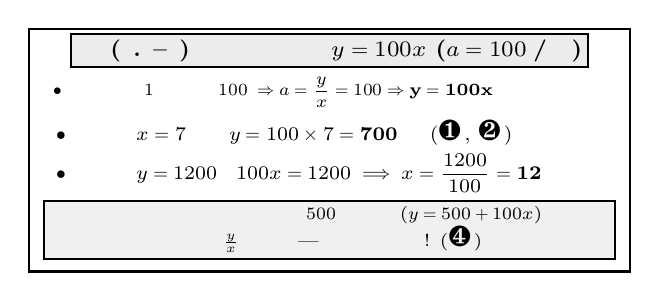
\begin{tikzpicture}[x=0.96cm, y=0.92cm, every node/.style={font=\scriptsize, text=black}]
  \draw[black, line width=0.95pt] (0,0) rectangle (7.95,3.35);
  \node[fill=gray!15, draw=black, line width=0.6pt, inner sep=2pt, font=\footnotesize\bfseries] at (3.975,3.05) {គំរូ (ទំ.២៧–២៨)៖ ប្រាក់ពិន័យបណ្ណាល័យ $y = 100x$ ($a = 100\text{៛/ថ្ងៃ}$)};

  \node[anchor=west, font=\fontsize{6.2pt}{8pt}\selectfont] at (0.20,2.48) {$\bullet$ \textbf{មេគុណសមាមាត្រ៖} $1$ ថ្ងៃ ពិន័យ $100\text{៛} \Rightarrow a = \dfrac{y}{x} = 100 \Rightarrow \mathbf{y = 100x}$};
  \node[anchor=west] at (0.24,1.92) {$\bullet$ \textbf{ករណីស្គាល់ $x=7$ ថ្ងៃ៖} $y = 100 \times 7 = \mathbf{700\text{៛}}$ \quad (\cnum{1}, \cnum{2})};
  \node[anchor=west] at (0.24,1.36) {$\bullet$ \textbf{ករណីស្គាល់ $y=1200\text{៛}$៖} $100x = 1200 \implies x = \dfrac{1200}{100} = \mathbf{12\text{ ថ្ងៃ}}$};
  \draw[black, line width=0.7pt, fill=gray!12] (0.20,0.18) rectangle (7.75,0.98);
  \node[align=center, font=\fontsize{6.3pt}{7.8pt}\selectfont] at (3.975,0.58) {\textbf{ប្រៀបធៀបអន្ទាក់៖} បើមានថ្លៃចុះឈ្មោះថេរ $500\text{៛}$ បូកបន្ថែម ($y=500+100x$)\\នោះផលធៀប $\frac{y}{x}$ \textbf{លែងថេរហើយ} — មិនមែនសមាមាត្រស្របទេ! (\cnum{4})};
\end{tikzpicture}}

% ៤. E5 Diagnostic Options A-D
\newcommand{\figExitCardsPROPA}{%
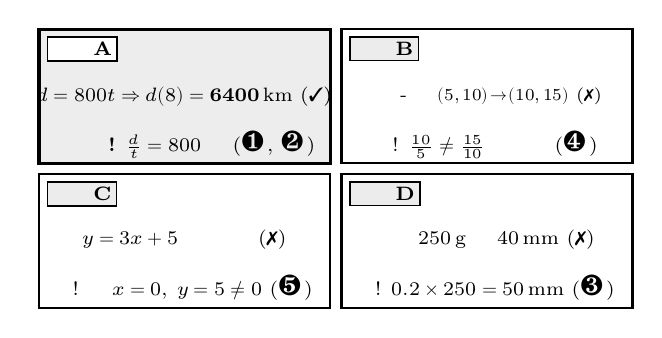
\begin{tikzpicture}[x=0.96cm, y=0.92cm, every node/.style={font=\scriptsize, text=black}]
  \draw[black, line width=1.1pt, fill=gray!14] (0,2.00) rectangle (3.85,3.85);
  \node[anchor=north west, fill=white, draw=black, line width=0.6pt, inner sep=1.8pt] at (0.10,3.75) {\textbf{ជម្រើស \en{A}}};
  \node at (1.925,2.92) {$d = 800t \Rightarrow d(8) = \mathbf{6400\unit{km}}$ (\ding{51})};
  \node at (1.925,2.25) {\textbf{ត្រឹមត្រូវ!} $\frac{d}{t}=800$ ថេរ (\cnum{1}, \cnum{2})};

  \draw[black, line width=0.9pt] (4.00,2.00) rectangle (7.85,3.85);
  \node[anchor=north west, fill=gray!15, draw=black, line width=0.6pt, inner sep=1.8pt] at (4.10,3.75) {\textbf{ជម្រើស \en{B}}};
  \node[font=\fontsize{6.1pt}{8pt}\selectfont] at (5.925,2.92) {អាយុបង-ប្អូន $(5,10)\!\to\!(10,15)$ (\ding{55})};
  \node at (5.925,2.25) {ខុស! $\frac{10}{5}\ne\frac{15}{10}$ អន្ទាក់បូក (\cnum{4})};

  \draw[black, line width=0.9pt] (0,0) rectangle (3.85,1.85);
  \node[anchor=north west, fill=gray!15, draw=black, line width=0.6pt, inner sep=1.8pt] at (0.10,1.75) {\textbf{ជម្រើស \en{C}}};
  \node at (1.925,0.95) {$y = 3x + 5$ សមាមាត្រស្រប (\ding{55})};
  \node at (1.925,0.28) {ខុស! ពេល $x=0,\; y=5\ne 0$ (\cnum{5})};

  \draw[black, line width=0.9pt] (4.00,0) rectangle (7.85,1.85);
  \node[anchor=north west, fill=gray!15, draw=black, line width=0.6pt, inner sep=1.8pt] at (4.10,1.75) {\textbf{ជម្រើស \en{D}}};
  \node at (5.925,0.95) {រ៉ឺស័រ $250\unit{g}$ លូត $40\unit{mm}$ (\ding{55})};
  \node at (5.925,0.28) {ខុស! $0.2\times 250 = 50\unit{mm}$ (\cnum{3})};
\end{tikzpicture}}

\begin{document}
\fontsize{10pt}{15.2pt}\selectfont

% -------------------- ក្បាលកិច្ចតែងការ --------------------
\begin{center}
  {\muol\fontsize{11pt}{16pt}\selectfont ព្រះរាជាណាចក្រកម្ពុជា}\\[2pt]
  {\muol\fontsize{10pt}{15pt}\selectfont ជាតិ សាសនា ព្រះមហាក្សត្រ}\\[1pt]
  \khmflourish
\end{center}

\vspace{-24pt}
{\muol\fontsize{9.5pt}{12.5pt}\selectfont
មន្ទីរអប់រំ យុវជន និងកីឡា ខេត្តកំពង់ធំ\\
ការិយាល័យអប់រំ យុវជន និងកីឡា ស្រុកកំពង់ស្វាយ\\
អនុវិទ្យាល័យព្រះក្រសាំង}

\vspace{1pt}
\begin{center}
  {\muol\fontsize{10pt}{14pt}\selectfont កិច្ចតែងការបង្រៀន}
\end{center}
\vspace{0pt}

% -------------------- ព័ត៌មានទូទៅ --------------------
{\renewcommand{\arraystretch}{0.98}
\hspace*{3.1cm}%
\begin{tabular}{@{}l l L{11.0cm}@{}}
  - \hspace{0.35cm} មុខវិជ្ជា & : & គណិតវិទ្យា ថ្នាក់ទី៨ (ពីជគណិត) \\
  - \hspace{0.35cm} ចំណងជើងមេរៀន & : & មេរៀនទី៣៖ ទំហំសមាមាត្រ និងភាគរយ \\
  - \hspace{0.35cm} ចំណងជើងរង & : & ១.១. ទំហំសមាមាត្រស្រប (សៀវភៅពុម្ព ទំ.២៧–២៨ និងលំហាត់ \#6, \#7, \#10 ទំ.៤០–៤១) \\
  - \hspace{0.35cm} រយៈពេល & : & ១ ម៉ោងសិក្សា (៥០ នាទី) \\
  - \hspace{0.35cm} បង្រៀនដោយ & : & ហុក ប៊ុនថែន \\
  - \hspace{0.35cm} កាលបរិច្ឆេទ & : & ថ្ងៃសៅរ៍ ទី២១ ខែវិច្ឆិកា ឆ្នាំ២០២៦ \\
\end{tabular}

\vspace{2pt}

% -------------------- I. វត្ថុបំណង --------------------
\textbf{I.} {\muol វត្ថុបំណង}\\[1pt]
\hspace*{0.55cm}%
\begin{tabular}{@{}l l L{14.2cm}@{}}
  \wcirc \hspace{0.25cm} វិជ្ជាសម្បទា & : & សិស្សប្រាប់និយមន័យទំហំសមាមាត្រស្របតាមរយៈផលធៀបថេរ $\dfrac{y}{x} = a$ (ឬ $y = ax$ ដែល $a\neq 0$ ជាមេគុណសមាមាត្រ) និងបែងចែកដាច់ពីទំនាក់ទំនងបូកបន្ថែម ។ \\
  \wcirc \hspace{0.25cm} បំណិនសម្បទា & : & សិស្សពិនិត្យតារាងតម្លៃ កំណត់មេគុណសមាមាត្រ $a$ សរសេរសមីការ $y = ax$ និងដោះស្រាយចំណោទជីវភាព (រ៉ឺស័រ ប្រាក់ពិន័យ និងល្បឿនយន្តហោះ ទំ.២៧–២៨, ៤០–៤១) លើសន្លឹកកិច្ចការ ។ \\
  \wcirc \hspace{0.25cm} ចរិយាសម្បទា & : & សិស្សមានទម្លាប់ផ្ទៀងផ្ទាត់ផលធៀប $\dfrac{y}{x}$ គ្រប់ជួរឈរមុនសន្និដ្ឋាន និងឱ្យតម្លៃលើការអនុវត្តទំហំសមាមាត្រក្នុងរូបវិទ្យា និងជីវភាពរស់នៅ ។ \\
\end{tabular}

\vspace{2pt}

% -------------------- II. សម្ភារៈឧបទេស --------------------
\textbf{II.} {\muol សម្ភារៈឧបទេស}\\[1pt]
\hspace*{0.55cm}$\bullet$ \hspace{0.35cm} សៀវភៅសិក្សាគោលគណិតវិទ្យាថ្នាក់ទី៨ (ទំ.២៧–២៨, ៤០–៤១) ក្ដារខៀន ដីស និងសន្លឹកកិច្ចការសិស្ស ស-ខ្មៅ (\en{Worksheet\_PROP1} ទំព័រ ១–២ គ្មានស្លាយ \en{LCD})

\vspace{2pt}

% -------------------- III. វិធីសាស្រ្តបង្រៀន --------------------
\textbf{III.} {\muol វិធីសាស្រ្តបង្រៀន}\\[1pt]
\hspace*{0.45cm}%
\begin{tabular}{@{}l l L{14.85cm}@{}}
  $\bullet$ \hspace{0.25cm} គោលវិធី & : & សិស្សមជ្ឈមណ្ឌល (បង្រៀនតាមសន្លឹកកិច្ចការស៊ើបអង្កេត និងក្ដារខៀន គ្មាន \en{LCD}) \\
  $\bullet$ \hspace{0.25cm} យុទ្ធវិធីបង្រៀន & : & គំរូ \en{5Es} រួមបញ្ចូលតារាងត្រួតពិនិត្យផលធៀបថេរ $\dfrac{y}{x}=a$ ប្រឆាំងអន្ទាក់បូកបន្ថែម (\en{Constant-Quotient vs. Additive Trap}) \\
\end{tabular}
}

\vspace{2pt}

% -------------------- IV. ដំណើរការបង្រៀន --------------------
\textbf{IV.} {\muol ដំណើរការបង្រៀន}

\vspace{1pt}

\renewcommand{\arraystretch}{1.15}
\begin{longtable}{|L{5.50cm}|L{7.90cm}|L{4.80cm}|}
\hline
\rowcolor{headgray}
\multicolumn{1}{|c|}{\muol សកម្មភាពគ្រូ} &
\multicolumn{1}{c|}{\muol ខ្លឹមសារមេរៀន} &
\multicolumn{1}{c|}{\muol សកម្មភាពសិស្ស} \\
\hline
\endfirsthead
\hline
\endhead
\hline
\endfoot
\hline
\endlastfoot

% ==================== ជំហានទី១ (2min) ====================
\stepheader{ជំហានទី១ \enbf{(}រដ្ឋបាលថ្នាក់\enbf{)}}
$\bullet$ ពិនិត្យអវត្តមាន អនាម័យ និងសណ្ដាប់ធ្នាប់ថ្នាក់រៀន
&
$\bullet$ រដ្ឋបាលថ្នាក់ និងការរៀបចំដៃគូសិក្សា
&
$\circ$ ប្រធានថ្នាក់រាយការណ៍អវត្តមាន \\[3pt]

$\bullet$ ចែក \textbf{សន្លឹកកិច្ចការសិស្ស (\en{Worksheet\_PROP1})} ម្នាក់ ១ សន្លឹក (ផ្កាប់ទុកសិន)
&
$\bullet$ សន្លឹកកិច្ចការសិស្ស ស-ខ្មៅ (\en{Worksheet\_PROP1} ទំព័រ ១–២)
&
$\circ$ ទទួលសន្លឹកកិច្ចការ និងត្រៀមសម្ភារៈសរសេរ \\
\hline

% ==================== ជំហានទី២ (9min: <=3 + 3 + E1 3) ====================
\stepheader{ជំហានទី២ \enbf{(}កិច្ចការផ្ទះ \enbf{+} ទំនាក់ទំនងមេរៀនថ្មី\enbf{)}}
\ditem \textbf{កំណែកិច្ចការផ្ទះ ($\le 3\unit{min}$)} \timenote{(កុំសរសេរវែង)} \par
$\bullet$ ហៅសិស្ស ២ នាក់ឡើងសរសេរចម្លើយលំហាត់ \#16 និង \#17 (ទំ.២៦) លើក្ដារខៀន
&
{\centering\redsub{កំណែកិច្ចការផ្ទះមេរៀនទី២ (ទំ.២៦ \#16 និង \#17)}\par} \par
$\bullet$ \textbf{\#16៖} $\sqrt{441}=21,\; \sqrt{784}=28,\; \sqrt{1225}=35,\; \sqrt{1764}=42$ \par
$\bullet$ \textbf{\#17៖} ផ្ទៀងឫសការេនៃទសភាគ និងប្រភាគតាមក្បួនខ្ទង់ពាក់កណ្ដាល
&
$\circ$ ផ្ទៀងផ្ទាត់ចម្លើយក្នុងសៀវភៅកិច្ចការផ្ទះ \\[3pt]

\ditem \textbf{រំលឹកមេរៀនទាក់ទង (3min)} \par
$\bullet$ សួររហ័ស៖ សម្រួលប្រភាគ $\dfrac{10}{50}, \dfrac{20}{100}, \dfrac{30}{150}$ ជាទសភាគ និងរំលឹករូបមន្តចម្ងាយចរ
&
{\centering\redsub{រំលឹកផលធៀបស្មើគ្នា និងរូបមន្តចម្ងាយចរ}\par} \par
$\bullet$ $\dfrac{10}{50} = \dfrac{20}{100} = \dfrac{30}{150} = \dfrac{1}{5} = 0.2$ \;;\; ចម្ងាយចរ $d = v \times t$
&
$\circ$ សម្រួលប្រភាគរហ័ស និងប្រាប់រូបមន្ត $d = v\times t$ \\[3pt]

\fiveE{E1 - Engage (3min)} \timenote{(កុំទាន់ផ្ដល់ចម្លើយ)} \par
\ditem \textbf{«បេសកកម្មជញ្ជីងរ៉ឺស័រ ទល់នឹង អន្ទាក់អាយុបងប្អូន» (ទំ.២៧)} \par
$\bullet$ ឱ្យសិស្សបើកសន្លឹកកិច្ចការទំព័រ ១ គូសធីកទស្សន៍ទាយលើសំណួរ ២
&
{\centering\redsub{បេសកកម្ម E1៖ រ៉ឺស័រយឺត ទល់នឹង អាយុបងប្អូន}\par} \par
$\bullet$ \textbf{សំណួរ ១ (ទំ.២៧)៖} រ៉ឺស័រព្យួរ $50\unit{g}$ លូត $10\unit{mm}$, ព្យួរ $100\unit{g}$ លូត $20\unit{mm}$ — បើព្យួរ $250\unit{g}$ តើលូត $40\unit{mm}$ ឬ $50\unit{mm}$? \par
$\bullet$ \textbf{សំណួរ ២៖} ប្អូន $5$ ឆ្នាំ បង $10$ ឆ្នាំ ; ៥ ឆ្នាំក្រោយ ប្អូន $10$ បង $15$ — តើសមាមាត្រស្របឬទេ?
&
$\circ$ គូសធីកទស្សន៍ទាយលើសន្លឹកកិច្ចការទំព័រ ១ \\[3pt]

&
\cfig{\figEngagePROPA}
& \\[3pt]

$\bullet$ ស្រង់ចំនួនដៃសិស្សកត់លើក្ដារខៀន (មិនទាន់ប្រាប់ចម្លើយត្រូវ)
&
$\bullet$ ស្ថិតិទស្សន៍ទាយ៖ $40\unit{mm}$ ទល់នឹង $50\unit{mm}$ ; សមាមាត្រ ទល់នឹង មិនសមាមាត្រ
&
$\circ$ លើកដៃបង្ហាញការទស្សន៍ទាយ \\
\hline

% ==================== ជំហានទី៣ (17min: E2 11m + E3 6m) ====================
\stepheader{ជំហានទី៣ \enbf{(}ខ្លឹមសារមេរៀនថ្មី\enbf{)}}
\fiveE{E2 - Explore (11min)} \par
$\bullet$ សរសេរចំណងជើងមេរៀនទី៣ និងចំណងជើងរងលើក្ដារខៀន
&
\textbf{មេរៀនទី៣៖ ទំហំសមាមាត្រ និងភាគរយ — ១.១. ទំហំសមាមាត្រស្រប} (ទំ.២៧–២៨)
&
$\circ$ កត់ចំណងជើងចូលសៀវភៅ \\[3pt]

\ditem \textbf{សកម្មភាព ១៖ ពិសោធន៍តារាងរ៉ឺស័រ \en{POE 1} (6min, ទំ.២៧ ផ្នែកទី១-ក)} \par
$\bullet$ ឱ្យដៃគូគណនាផលធៀប $\dfrac{y}{x}$ គ្រប់ជួរឈរនៃតារាងរ៉ឺស័រលើសន្លឹកកិច្ចការ
&
{\centering\textbf{សកម្មភាព ១ (\en{POE 1})៖ តារាងរ៉ឺស័រ (ទំ.២៧)}\par} \par
$\bullet$ $\dfrac{10}{50} = \dfrac{20}{100} = \dfrac{30}{150} = \dfrac{50}{250} = 0.2$ (ថេរជានិច្ច!) \par
$\bullet$ គេថាប្រវែងលូត $y$ \textbf{សមាមាត្រស្រប}នឹងទម្ងន់ $x$ តាមសមីការ $\mathbf{y = 0.2x}$
&
$\circ$ គណនាផលធៀប $\frac{y}{x}$ ទាំង ៤ ជួរឈរ និងរកឃើញតម្លៃថេរ $0.2$ \\[3pt]

\ditem \textbf{សកម្មភាព ២៖ បំបែកអន្ទាក់ «កើនទាំងពីរ» \en{POE 2} (5min, ផ្នែកទី១-ខ)} \par
$\bullet$ ឱ្យដៃគូប្រៀបធៀបតារាងប្រាក់ពិន័យបណ្ណាល័យ នឹងតារាងអាយុបងប្អូន
&
{\centering\textbf{សកម្មភាព ២ (\en{POE 2})៖ ផលធៀបថេរ ទល់នឹង អន្ទាក់បូកថេរ}\par} \par
$\bullet$ \textbf{តារាង ក (ពិន័យបណ្ណាល័យ)៖} $\frac{100}{1} = \frac{200}{2} = \frac{500}{5} = 100$ (ថេរ $\implies$ សមាមាត្រស្រប \ding{51}) \par
$\bullet$ \textbf{តារាង ខ (អាយុបងប្អូន)៖} $\frac{10}{5} = 2 \neq \frac{15}{10} = 1.5$ (មិនថេរ $\implies$ មិនសមាមាត្រស្រប \ding{55})
&
$\circ$ ពិនិត្យផលធៀប $\frac{y}{x}$ លើតារាងទាំងពីរ និងរកឃើញអន្ទាក់បូកថេរ \\[3pt]

&
\cfig{\figSpringPROPA}
& \\[3pt]

% --- E3 Explain (6min) ---
\fiveE{E3 - Explain (6min)} \par
\ditem \textbf{បង្គុំនិយមន័យ «ជាទូទៅ» (ទំ.២៧) និងធនាគារហេតុផល (ផ្នែកទី២)} \par
$\bullet$ ឱ្យសិស្សបង្គុំប្រអប់ \textbf{ជាទូទៅ (ទំ.២៧)} និងពន្យល់អត្ថន័យមេគុណសមាមាត្រ $a$
&
$\bullet$ \textbf{ជាទូទៅ (ទំ.២៧)៖} ប្រសិនបើទំហំ $y$ សមាមាត្រស្របនឹងទំហំ $x$ គេបាន៖ \par
{\centering\graybox{$\dfrac{y}{x} = a$ \;;\; $y = ax$ \;($a \neq 0$)}\par} \par
ដែលចំនួនថេរ $a$ ហៅថា \textbf{មេគុណសមាមាត្រ} ។
&
$\circ$ បំពេញប្រអប់ «ជាទូទៅ» លើសន្លឹកកិច្ចការ និងកត់ចូលសៀវភៅ \\[3pt]

$\bullet$ សង្ខេប \textbf{ធនាគារហេតុផល \cnum{1}--\cnum{3}} អំពីនិយមន័យ មេគុណសមាមាត្រ និងពហុគុណ
&
\textbf{ធនាគារហេតុផល \en{B\&W} (\cnum{1}--\cnum{5})៖} \par
\cnum{1} និយមន័យសមាមាត្រស្រប៖ $\dfrac{y}{x} = a$ (ថេរគ្រប់គូតម្លៃ) $\iff y = ax$ ($a\neq 0$) \par
\cnum{2} មេគុណសមាមាត្រ $a$៖ តាងតម្លៃនៃ $y$ ត្រូវនឹង $1$ ឯកតានៃ $x$ ($a = \frac{y}{x}$) \par
\cnum{3} លក្ខណៈពហុគុណ៖ បើ $x$ គុណនឹង $k$ ($k\neq 0$) នោះ $y$ ក៏ត្រូវគុណនឹង $k$ ដែរ
&
$\circ$ ផ្ទៀងផ្ទាត់ហេតុផល \cnum{1}--\cnum{3} លើសន្លឹកកិច្ចការ \\[3pt]

$\bullet$ សង្ខេប \textbf{ធនាគារហេតុផល \cnum{4}--\cnum{5}} សម្រាប់បំបែកអន្ទាក់បូកថេរ និងលក្ខខណ្ឌគល់ $(0,0)$
&
\cnum{4} អន្ទាក់បូកថេរ៖ គ្រាន់តែកើនទាំងពីរ ($y = x + c,\; c\neq 0$) មិនមែនសមាមាត្រស្របទេ! \par
\cnum{5} លក្ខខណ្ឌគល់ $(0,0)$៖ ក្នុងរូបមន្ត $y = ax$ ពេល $x = 0$ ត្រូវបាន $y = 0$ ជានិច្ច
&
$\circ$ ផ្ទៀងផ្ទាត់ហេតុផល \cnum{4}--\cnum{5} លើសន្លឹកកិច្ចការ \\
\hline

% ==================== ជំហានទី៤ (20min: E4 10m + E5 10m) ====================
\stepheader{ជំហានទី៤ \enbf{(}ពង្រីកចំណេះដឹង និងវាយតម្លៃ\enbf{)}}
\fiveE{E4 - Elaborate (10min)} \par
\ditem \textbf{លំហាត់គំរូ (ទំ.២៧–២៨ — សន្លឹកកិច្ចការ ទំព័រ ២ ផ្នែកទី៣)} \par
$\bullet$ ដឹកនាំដោះស្រាយ \textbf{លំហាត់គំរូប្រាក់ពិន័យបណ្ណាល័យ (ទំ.២៧–២៨)} លើក្ដារខៀន
&
{\muol លំហាត់គំរូទី ១} \textbf{(ទំ.២៧–២៨ — ពិន័យបណ្ណាល័យ $100\text{៛}$ ក្នុង ១ ថ្ងៃ)៖} \par
$\bullet$ \textbf{ក.} មេគុណសមាមាត្រ $a = 100 \implies$ សមីការ $\mathbf{y = 100x}$ (\cnum{1}, \cnum{2}) \par
$\bullet$ \textbf{ខ.} បើហួសកំណត់ $x = 7$ ថ្ងៃ $\implies y = 100\times 7 = \mathbf{700\text{៛}}$ (\cnum{3}) \par
$\bullet$ \textbf{គ.} បើបង់ប្រាក់ពិន័យ $y = 1200\text{៛} \implies x = \dfrac{1200}{100} = \mathbf{12\text{ ថ្ងៃ}}$ (\cnum{1})
&
$\circ$ បំពេញជំហានលំហាត់គំរូទី ១ លើសន្លឹកកិច្ចការ \\[3pt]

$\bullet$ ដឹកនាំ \textbf{លំហាត់គំរូទី ២ (ពិនិត្យតារាងតម្លៃ លំនាំ \#6ក, ខ ទំ.៤០)}
&
{\muol លំហាត់គំរូទី ២} \textbf{(ពិនិត្យតារាងតម្លៃ លំនាំ \#6 ទំ.៤០)៖} \par
$\bullet$ \textbf{ក.} $(2,6),(4,12),(7,21) \implies \frac{6}{2}=\frac{12}{4}=\frac{21}{7}=3$ ថេរ $\implies \mathbf{y = 3x}$ (\cnum{1}) \par
$\bullet$ \textbf{ខ.} $(1,4),(2,7),(3,10) \implies \frac{4}{1}=4 \neq \frac{7}{2}=3.5 \implies$ \textbf{មិនសមាមាត្រស្រប} (\cnum{4})
&
$\circ$ គណនាផលធៀប $\frac{y}{x}$ ដើម្បីសម្រេចថាសមាមាត្រ ឬមិនសមាមាត្រ \\[3pt]

&
\cfig{\figLibraryPROPA}
& \\[3pt]

$\bullet$ សួរសំណួរឆ្លុះបញ្ចាំង \textbf{\en{EIA Looking-Back} (៣០ វិនាទី)}
&
\textbf{\en{EIA Looking-Back}៖} «បើឈ្នួលម៉ូតូឌុបគិតថ្លៃចាប់ផ្ដើម $2000\text{៛}$ បូក $1500\text{៛}$ ក្នុង $1\unit{km}$ ($y = 2000 + 1500x$) តើ $y$ សមាមាត្រស្របនឹង $x$ ដែរឬទេ? ហេតុអ្វី?»
&
$\circ$ ឆ្លើយ៖ «ទេ! ព្រោះពេល $x=0,\; y=2000\neq 0$ និង $\frac{y}{x}$ មិនថេរ!» \\[3pt]

% --- E5 Evaluate (10min) ---
\fiveE{E5 - Evaluate (10min)} \par
\ditem \textbf{ហ្វឹកហាត់ជាដៃគូលើ «ប្រតិបត្តិ» (6min, ទំ.២៨ — ផ្នែកទី៤-ក)} \par
$\bullet$ ឱ្យដៃគូធ្វើ \textbf{ប្រតិបត្តិ ១ (ទំ.២៨ លើ — ល្បឿនយន្តហោះ $800\unit{km/h}$)}
&
{\muol លំហាត់ប្រតិបត្តិ} \textbf{(ទំ.២៨ លើ និងពង្រឹង \#7 ទំ.៤១)៖} \par
$\bullet$ \textbf{១) ប្រតិបត្តិ (ទំ.២៨)៖} យន្តហោះហោះបាន $800\unit{km}$ ក្នុង $1\unit{h} \implies \mathbf{d = 800t}$ (\cnum{2}) \par
$\bullet$ ពេល $t = 8\unit{h} \implies d = \mathbf{6400\unit{km}}$ ; ចម្ងាយ $2000\unit{km} \implies t = \dfrac{2000}{800} = \mathbf{2.5\unit{h}}$
&
$\circ$ គណនាចម្ងាយ និងរយៈពេលហោះលើសន្លឹកកិច្ចការ \\[3pt]

$\bullet$ ឱ្យដៃគូធ្វើ \textbf{ពង្រឹង \#7 (ទំ.៤១)} រួចប្ដូរសន្លឹកផ្ទៀងផ្ទាត់ (\en{Pause-Review})
&
$\bullet$ \textbf{២) ពង្រឹង (\#7 ទំ.៤១)៖} បើ $y$ សមាមាត្រស្របនឹង $x$ ហើយពេល $x=4 \Rightarrow y=12$ នោះ $a = \frac{12}{4} = 3 \implies \mathbf{y = 3x}$ ; ពេល $x=9 \Rightarrow y = \mathbf{27}$ (\cnum{1}, \cnum{3})
&
$\circ$ បំពេញពង្រឹង \#7 រួចប្ដូរសន្លឹកផ្ទៀងផ្ទាត់ជាមួយដៃគូ \\[3pt]

$\bullet$ បិទបេសកកម្ម \en{E1} និងឱ្យសិស្សវិនិច្ឆ័យ \textbf{ជម្រើស \en{A--D}} + \textbf{\en{Exit Check}} (4min)
&
$\bullet$ \textbf{បិទបេសកកម្ម \en{E1}៖} រ៉ឺស័រព្យួរ $250\unit{g}$ លូត $50\unit{mm}$ ; អាយុបងប្អូនមិនសមាមាត្រស្របទេ ។ \par
$\bullet$ \textbf{វិនិច្ឆ័យជម្រើស \en{A--D} លើសន្លឹកកិច្ចការ៖}
&
$\circ$ ផ្ទៀងចម្លើយ \en{E1} និងគូសវង់ជម្រើសត្រូវ \en{A} \\[3pt]

&
\cfig{\figExitCardsPROPA}
& \\[3pt]

$\bullet$ ពិនិត្យរហ័សលើសំបុត្រចេញ ៣ ខ្ទង់នៅបាតសន្លឹកកិច្ចការ (៦០ វិនាទី)
&
$\bullet$ \textbf{\en{Exit Check}៖} ១) $x=5, y=35 \Rightarrow a = 7$ ; ២) រូបមន្ត $y = 7x$ ; ៣) ពេល $x=8 \Rightarrow y = 56$ ។
&
$\circ$ បំពេញសំបុត្រចេញទាំង ៣ ខ្ទង់ដោយខ្លួនឯង \\
\hline

% ==================== ជំហានទី៥ (<=2min) ====================
\stepheader{ជំហានទី៥ \enbf{(}កិច្ចការផ្ទះ \enbf{+} បណ្ដាំផ្ញើ\enbf{)}}
\timenote{ចំណាយពេលឱ្យតិចបំផុតកុំឱ្យលើស 2min} \par
$\bullet$ ណែនាំកិច្ចការផ្ទះនៅបាតសន្លឹកកិច្ចការ (សៀវភៅពុម្ព ទំ.៤០–៤១ លំហាត់ \#6ក-គ, \#7 និង \#10)
&
{\centering{\muol កិច្ចការផ្ទះ} \textbf{(សៀវភៅគោល ទំ.៤០–៤១ លំហាត់ \#6ក-គ, \#7 និង \#10)៖}\par} \par
$\bullet$ \textbf{លំហាត់ \#6 (ក, ខ, គ ទំ.៤០)៖} ពិនិត្យតារាងតើ $y$ សមាមាត្រស្របនឹង $x$ ឬទេ និងរកមេគុណសមាមាត្រ $a$ \par
$\bullet$ \textbf{លំហាត់ \#7 និង \#10 (ទំ.៤១)៖} សរសេរសមីការ $y = ax$ និងគណនាតម្លៃដែលខ្វះក្នុងចំណោទជីវភាព (ផ្ទៀងផលធៀបថេរ $\frac{y}{x}=a$ គ្រប់ជំហាន)
&
$\circ$ កត់ចំណាំលំហាត់ \#6, \#7 និង \#10 សម្រាប់ធ្វើនៅផ្ទះ \\[3pt]

$\bullet$ ផ្ដាំផ្ញើឱ្យអានមុន \textbf{១.២. លក្ខណៈនៃសមាមាត្រស្រប (ទំ.២៨–៣០)}
&
$\bullet$ \textbf{មេរៀនបន្ទាប់៖} អានមុន \textbf{១.២. លក្ខណៈទី ១ និងលក្ខណៈទី ២ នៃសមាមាត្រស្រប (ទំ.២៨–៣០)} ។
&
$\circ$ កត់ចំណាំមេរៀនបន្ទាប់ និងជម្រាបលាគ្រូ \\
\end{longtable}

\vspace{6pt}
\hfill
\begin{minipage}{10.5cm}
  {\centering
    ថ្ងៃសៅរ៍ ១២កើត ខែកត្តិក ឆ្នាំមមី អដ្ឋស័ក ពុទ្ធសករាជ ២៥៧០\\[2pt]
    កំពង់ស្វាយ, ថ្ងៃទី២១ ខែវិច្ឆិកា ឆ្នាំ២០២៦\\[3pt]
    {\muol គ្រូបង្រៀន}\par}
  \vspace{28pt}
  \hfill{\muol ហុក ប៊ុនថែន}\hspace*{1.4cm}
\end{minipage}

\end{document}
